\documentclass[11pt]{article}\usepackage[]{graphicx}\usepackage[]{color}
%% maxwidth is the original width if it is less than linewidth
%% otherwise use linewidth (to make sure the graphics do not exceed the margin)
\makeatletter
\def\maxwidth{ %
  \ifdim\Gin@nat@width>\linewidth
    \linewidth
  \else
    \Gin@nat@width
  \fi
}
\makeatother

\definecolor{fgcolor}{rgb}{0.345, 0.345, 0.345}
\newcommand{\hlnum}[1]{\textcolor[rgb]{0.686,0.059,0.569}{#1}}%
\newcommand{\hlstr}[1]{\textcolor[rgb]{0.192,0.494,0.8}{#1}}%
\newcommand{\hlcom}[1]{\textcolor[rgb]{0.678,0.584,0.686}{\textit{#1}}}%
\newcommand{\hlopt}[1]{\textcolor[rgb]{0,0,0}{#1}}%
\newcommand{\hlstd}[1]{\textcolor[rgb]{0.345,0.345,0.345}{#1}}%
\newcommand{\hlkwa}[1]{\textcolor[rgb]{0.161,0.373,0.58}{\textbf{#1}}}%
\newcommand{\hlkwb}[1]{\textcolor[rgb]{0.69,0.353,0.396}{#1}}%
\newcommand{\hlkwc}[1]{\textcolor[rgb]{0.333,0.667,0.333}{#1}}%
\newcommand{\hlkwd}[1]{\textcolor[rgb]{0.737,0.353,0.396}{\textbf{#1}}}%

\usepackage{framed}
\makeatletter
\newenvironment{kframe}{%
 \def\at@end@of@kframe{}%
 \ifinner\ifhmode%
  \def\at@end@of@kframe{\end{minipage}}%
  \begin{minipage}{\columnwidth}%
 \fi\fi%
 \def\FrameCommand##1{\hskip\@totalleftmargin \hskip-\fboxsep
 \colorbox{shadecolor}{##1}\hskip-\fboxsep
     % There is no \\@totalrightmargin, so:
     \hskip-\linewidth \hskip-\@totalleftmargin \hskip\columnwidth}%
 \MakeFramed {\advance\hsize-\width
   \@totalleftmargin\z@ \linewidth\hsize
   \@setminipage}}%
 {\par\unskip\endMakeFramed%
 \at@end@of@kframe}
\makeatother

\definecolor{shadecolor}{rgb}{.97, .97, .97}
\definecolor{messagecolor}{rgb}{0, 0, 0}
\definecolor{warningcolor}{rgb}{1, 0, 1}
\definecolor{errorcolor}{rgb}{1, 0, 0}
\newenvironment{knitrout}{}{} % an empty environment to be redefined in TeX

\usepackage{alltt}
%\documentclass[11pt]{scrartcl}
\usepackage{amsmath, amsfonts, amssymb}
\usepackage{adjustbox}
\usepackage{fullpage}
\usepackage{epsfig}
\usepackage{hyperref}
\hypersetup{
     colorlinks   = true,
     citecolor    = black
}
\hypersetup{linkcolor=black}

\usepackage{multicol}

\renewcommand{\baselinestretch}{1.4}
\usepackage{float}
\usepackage{wrapfig}

\usepackage{tikz}
\usetikzlibrary{shapes,arrows}


\title{Data exploration, quality control and statistical analyses of
  ChIP-exo experiments\vspace*{\fill}}

\author{Rene Welch\\Preliminary Examination\\Department of Statistics,
  University of Wisconsin-Madison}

\date{December 1st, 2015}

%% commmands
%\usepackage{Sweave}
\IfFileExists{upquote.sty}{\usepackage{upquote}}{}
\begin{document}

\newcommand{\sig}{\sigma^{70}}


\maketitle

\vspace*{\fill}

\textbf{Committee Members:}

\textbf{Professor S\"und\"uz Kele\c{s}}, Department of Statistics,
Department of Biostatistics and Medical Informatics

\textbf{Professor Karl Broman}, Department of Biostatistics and
Medical Informatics

\textbf{Professor Colin Dewey}, Department of Computer Sciences,
Department of Biostatistics and Medical Informatics

\textbf{Professor Christina Kendziorski}, Department of Biostatistics
and Medical Informatics

\textbf{Professor Ming Yuan}, Department of Statistics

\thispagestyle{empty}


\newpage

\tableofcontents

\newpage

\listoffigures

\newpage


\section*{Abstract}

ChIP-exo is a modification of the ChIP-seq protocol for high
resolution mapping of transcription factor binding sites. Although
many aspect of the ChIP-exo data analysis are similar to those of
ChIP-Seq, ChIP-exo presents a number of unique challenges. We present
a quality control pipeline that analyzes ChIP-exo's strand imbalance
and library complexity. Assessment of these biases and artifacts are
facilitated through diagnostic plots and summary statistical that
compare a large portion of the genome as partitioned into island with
high depth regions.

We systematically evaluated diverse aspects of ChIP-exo and found the
following characteristics: First, ChIP-exo's background is quite
different than ChIP-Seq's. Second, although often assumed in ChIP-exo
data analysis methods, the ``peak pair'' assumption doesn't hold
locally in real ChIP-exo data. Third, we compared Paired End (PE)
ChIP-Seq with ChIP-exo and found that both protocols are comparable in
resolution and sensitivity for closely located binding event, but as
the distance between binding event increases ChIP-exo shows higher
sensitivity than PE ChIP-Seq. Finally, for given fixed sequencing
depth, ChIP-exo provides higher sensitivity, specificity and spatial
resolution than PE ChIP-Seq.

% optimal strategies for
%     experimental design and analysis of ChIP-exo.


% We also systematically compare multiple ChIP-seq and ChIP-exo
% datasets to quantify differences between these two protocols. Our
% analysis indicate that spatial resolution of ChIP-exo is comparable to
% that of paired-end ChIP-seq and both of them are significantly better
% than resolution of single-end ChIP-seq. Furthermore, for a given fixed
% sequencing depth, ChIP-exo provides higher sensitivity, specificity,
% and spatial resolution than pairedend ChIP-seq.

%     In order to address these questions, we evaluated diverse aspects
%     of ChIP-exo and found the following characteristics of ChIP-exo
%     data. First, the background of ChIP-exo data is quite different
%     from that of ChIP-Seq data. However, sequence biases inherently
%     present in ChIP-Seq data still exist in ChIP-exo data. Second, in
%     ChIP-exo data, reads are located around binding sites much more
%     tightly and hence, it has potential for high resolution
%     identification of protein-DNA interaction sites, and also the
%     space to allocate the reads is greatly reduced. Third, although
%     often assumed in the ChIP-exo data analysis methods, the ``peak
%     pair'' assumption does not hold well in real ChIP-exo
%     data. Fourth, spatial resolution of ChIP-exo is comparable to that
%     of PET ChIP-Seq and both of them are significantly better than
%     resolution of SET ChIP-Seq. Finally, for given fixed sequencing
%     depth, ChIP-exo provides higher sensitivity, specificity and
%     spatial resolution than PET ChIP-Seq.

%     We provide a quality control pipeline which visually assess
%     ChIP-exo biases, library complexity and enrichment; and calculates
%     a signal-to-noise measure. Also, we updated dPeak (Chung et al.,
%     2012 \cite{dpeak}), which makes a striking balance in sensitivity,
%     specificity and spatial resolution for ChIP-exo data analysis.

\newpage

\section{Introduction}
\label{sec:intro}


ChIP-exo (Chromatin Immunopecipitation followed by exonuclease
digestion and next generation sequencing, Rhee and Pugh, 2011
\cite{exo1}) is the state-of-the-art experiment developed to attain
single base-pair resolution of protein binding site identification and
it is considered as a powerful alternative to popularly used ChIP-Seq
(Chromatin Immunoprecipitation coupled with next generation
sequencing) assay.

While the number of produced ChIP-exo data keeps increasing,
characteristics of ChIP-exo data are not fully investigated
yet. First, DNA libraries generated by the ChIP-exo protocol seem to
be less complex than the libraries generated by ChIP-Seq (Mahony et
al., 2015 \cite{exo_review}), i.e. the number of positions to which
the reads can be aligned has been reduced due to the exonuclease
digestion. Second, although the are roughly the same amount of reads
in both strands, locally there may be more reads in one strand than in
the other. To address this challenges, we suggest a collection of
quality control visualizations to understand which of this biases are
present in ChIP-exo data and globally assess the enrichment and
library complexity of a ChIP-exo sample.We gathered ChIP-exo data from
diverse organisms: CTCF factor in human \cite{exo1}; ER factor in
human and FoxA1 factor in mouse (Serandour et al., 2013
\cite{exoillumina}); and generated $\sig$ factor in Escherichia Coli
(\emph{E. Coli}) under aerobic ($ + O_2$) condition, and treated by
rifampicin by 0 and 20 minutes (courtesy of Professor Robert Landick's
lab).
% While the number of produced ChIP-exo data keeps increasing,
% characteristics of ChIP-exo data and its analysis are not fully
% investigated yet, including issues of sequence biases inherent to
% ChIP-exo data, choice of optimal statistical methods, and
% determination of optimal sequencing depth. However, currently the
% number of available ChIP-exo data is still limited and their
% sequencing depths are still insufficient for such investigation.

Most of current ChIP-Seq QC guidelines (Landt et al., 2012
\cite{encode_qc}) may not be applicable on ChIP-exo, additionally to
our knowledge there are not established quality control pipelines for
ChIP-exo.Previous ChIP-exo analysis used ChIP-Seq samples to compare
the resolution between experiments (\cite{exo1}, \cite{exo2},
\cite{exoillumina}); Carroll et al., 2014 \cite{carroll.qc} studied
the use of the Strand-Cross Correlation (SCC) (Kharchenko et al., 2008
\cite{strandcc}) and showed that by filtering blacklisted regions the
estimation of the SCC is improved. However, this method requires to
know blacklisted regions in advance which may not be available,
additionally using SCC may not be useful since the peaks that are
attained at the read and fragment length are confused in a typical
ChIP-exo SCC curve.  In our pipeline we propose two out-the-shelf
analysis: an enrichment plot and the normalized local SCC coefficient.

In order to obtain the potential benefits of ChIP-exo on protein
binding site identification, it is critical to understand which are
the important characteristics of ChIP-exo data and to use algorithms
that could fully utilize information available in ChIP-exo data. Rhee
and Pugh, 2011 \cite{exo1} discussed that reads in the forward and
reverse strand might construct peak pairs around bound protein, of
which heights were implicitly assumed to be symmetric. Hence, they
used the ``peak pair method'' that predicts the midpoint of two modes
of peak pairs as potential binding site. Mace (Wang et al., 2014
\cite{mace}), CexoR (Madrigal, 2015 \cite{cexor}) and peakzilla
(Bardet et al., 2013 \cite{peakzilla}), recently developed ChIP-exo
data analysis methods, are also based on this peak pair
assumption. However, appropriateness of such assumption was not fully
evaluated in the literature yet.  Furthermore, it is still unknown
which factors could affect protein binding site identification using
ChIP-exo data. In order to address this problem, we investigated
various aspects of ChIP-exo data by contrasting them with their
respective ChIP-Seq experiments.

Currently, research on statistical methods for ChIP-exo data is still
in its very early stage. Although many methods have been proposed to
identify protein binding sites from ChIP-Seq data (reviewed by
Wilbanks and Facciotti, 2012 \cite{evaluation} and Pepke and Wold,
2009 \cite{computation}), such as MACS (Zhang et al., 2008
\cite{macs}), CisGenome (Ji et al., 2008 \cite{cisgenome}) and
MOSAiCS (Kuan et al., 2009 \cite{mosaics}), these approaches reveal
protein binding sites in lower resolution, i.e., at an interval of
hundreds to thousands of base pairs. Furthermore, they report only one
``mode'' or ``predicted binding location'' per peak. Hence, these
methods are not appropriate to evaluate the potential of ChIP-exo data
for high resolution identification of protein binding sites. More
recently, deconvolution algorithms such as Deconvolution (Lun et al.,
2009 \cite{csdeconv}), GEM (Guo et al., 2012 \cite{gem}, an improved
version of Guo et al., 2010 \cite{gps} ) and PICS (Zhang et al., 2010
\cite{pics}) have been proposed to identify binding sites in higher
resolution using ChIP-Seq data. However, most of them are still not
tailored for ChIP-exo and PE and SE ChIP-Seq data in a unified
framework and as a result, currently available methods are not
appropriate for fair comparison between ChIP-exo and ChIP-Seq. To
address these limitations, we developed an improved of dPeak (Chung et
al., 2013 \cite{dpeak}), a high resolution binding site identification
(deconvolution) algorithm that we previously developed for PE and SE
ChIP-Seq data, so that it can also handle ChIP-exo data. The dPeak
algorithm implements a probabilistic model that accurately describes
the ChIP-exo and ChIP-Seq data generation process.

In this work, we demonstrate that the ``peak pair'' assumption of Rhee
and Pugh \cite{exo1} does not hold well in real ChIP-exo
data. Furthermore, we found that when we analyze ChIP-exo data from
eukaryotic genomes, it is important to consider sequence biases
inherent to ChIP-exo data, such as mappability and GC content in order
to improve sensitivity and specificity of binding site
identification. We evaluated several method to identify binding events
and dPeak outperforms or performs competitively respect to GEM and
MACE when analyzing ChIP-exo data. More importantly, when comparable
number of reads is used for both ChIP-exo and ChIP-Seq, dPeak coupled
with ChIP-exo data provides outperform Paired End (PE) ChIP-Seq and
both significantly improve the resolution of protein binding site
identification compared to Single End (SE) ChIP-Seq.

\section{ChIP-exo and ChIP-Seq review}
\label{sec:exo}

\begin{wrapfigure}{l}{.4\textwidth}
\centering
\includegraphics{../figs/diagrams/ChIPexo_diagram.png}
\caption{ChIP-exo diagram. The only difference with ChIP-Seq is the
  second step, where an exonuclease enzyme is added and it digest the
  DNA fragments starting from the 5' end until it finds a crosslink
  protein (this Figure is taken from Furey, 2012 \cite{chipbeyond}).}
\label{fig:exo}
\end{wrapfigure}

ChIP-exo is based in a modification to the ChIP-seq protocol, where an
exonuclease enzyme is added and it digests the fragments starting by
the 5' ends and stops until it finds a protein that is crosslinked to
the DNA.

ChIP-exo experiments first capture millions of DNA fragments (150 -
250 bp in length) that the protein under study interacts with using
random fragmentation of DNA and a protein-specific antibody. Then,
exonuclease is introduced to trim 5' end of each DNA fragment to a
fixed distance from the bound protein. As a result, boundaries around
the protein of interest constructed with 5' ends of reads are located
much closed to bound protein compared to ChIP-Seq. This step is unique
to ChIP-exo and could potentially provide significantly higher spatial
resolution compared to ChIP-Seq. Finally, high throughput sequencing
of a small region (25 to 100 bp) at 5' end of each fragment generates
millions of reads or tags.

Since this protocol is a modification to ChIP-Seq, some of its
characteristics are still maintained in ChIP-exo while several new are
being found. Rhee and Pugh, 2011 \cite{exo1}, showed that ChIP-exo
generated fragments are located around the binding events more tightly
than ChIP-Seq generated fragments. Hence, it is of utmost importance
to understand how this new protocol works, specifically we focused on
understanding which biases are maintained from ChIP-Seq to ChIP-exo,
which biases are specific to ChIP-exo, how the current ChIP-Seq QC
guidelines behave in ChIP-exo and we developed a new QC pipeline
specific to ChIP-exo. A typical example is shown in Figure
\ref{fig:exo_example}, which shows the $\sig$ and $\beta'_f$ factors
(and the $\beta$ factor only on top) on a \emph{E. Coli} genome's
region: First, both regions show that the $\sig$ sample is enriched;
second the $\sig$ sample in the ChIP-exo panel shows that its
respective form in the ChIP-Seq panel may be form of more binding
events; and third, either of the $\beta$ factors show that the
complexity of the ChIP-exo libraries may be lower in some cases,
i.e. the peak is mapped with fewer positions. In \emph{E. Coli}
multiple promoters may be located close to each other, hence we may
suspect that the ChIP-Seq peak is occasioned by several promoter and
in the ChIP-exo panel we can observe that such is the case.

\begin{figure}[H]
  \centering
  \includegraphics[width = .8 \textwidth,page = 107]{/p/keles/ChIPexo/volume5/OpenClosedComplexes/figs/peaks/ChIPseq_ChIPexo_peaks_rif20.pdf}
  \caption{An example of a PE ChIP-Seq peak compared to
    ChIP-exo. $\sig$, $\beta$ and $\beta_f'$ are subunits of the
    transcription initiation complex in \emph{E. Coli}. Gene regions
    on the reverse strand are highlighted in light blue and the region
    was centered respect to ChIP-Seq $\sig$ summit. The library
    complexity is lower in ChIP-exo than in ChIP-Seq but the
    resolution is increased, this can be observed at the $\sig$ peak
    that for ChIP-exo was created as the combination of at least three
    ChIP-exo ``sub-peaks''.}
  \label{fig:exo_example}
\end{figure}

\subsection{Current Quality Control Measures for ChIP-Seq}
\label{sec:QC_chipseq}

We start our exploration by investigating the suitability of the
current state of the art QC pipeline for ChIP-Seq to ChIP-exo.

Table \ref{tab:qcbase} contains measures that are commonly used with
ChIP-Seq data. PBC stands for PCR bottleneck amplification and is
defined as the ratio between the number of positions to which exactly
one mapping read maps divided by the number of position to which at
least one mapping reads maps, the ENCODE project proposed a series of
ranges to interpret this quantity (which can be found in
\url{https://www.encodeproject.org/data-standards/2012-quality-metrics/}),
but it doesn't apply to ChIP-exo, if it did all the samples with
$\mbox{PBC} < 0.5$ should be reject due to be showing severe
bottlenecking. The normalized strand cross-correlation (NSC) is
defined as:

\[
\mbox{NSC} = \frac{ \max_\delta y(\delta)}{\min_\delta y(\delta)}
\]

where $y(\delta)$ is strand cross-correlation defined as in (\ref{scc}). 

\subsubsection{Strand Cross-Correlation}
\label{sec:scc}

The strand cross-correlation (SCC) was proposed by Kharchenko et al.,
2008 \cite{strandcc} and it may be one of the most used of the
ChIP-Seq QC metrics. The SCC curve is defined as:

\begin{align}
  y(\delta) = \sum_c w_c r\left[ n_c^+ \left(x + \frac{\delta}{2}
    \right), n_c^- \left( x- \frac{\delta}{2} \right)\right]
\label{scc}
\end{align}

where $y(\delta)$ is the SCC for a strand shift $\delta$, $r$ is the
Pearson correlation, $w_c$ is the proportion of reads mapped to
chromosome $c$ and $n_c^S$ is the read count vector for strand $S$ and
chromosome $c$.

\begin{figure}[H]
  \centering
  \includegraphics[width = \textwidth]{../figs/for_paper/SCC.png}
  \caption{SCC interpretation for ChIP-Seq from \cite{encode_qc}. In
    all panels, we observe shift $\delta$ vs SCC. The quality of
    ChIP-Seq is determined by the relative heights of the ``phantom
    peak'' and the local maximum when the shift is equal to the
    fragment length.}
  \label{fig:scc_landt}
\end{figure}

For ChIP-Seq data, the SCC will have two peaks: One when $\delta$ is
equal to read length and one when $\delta$ is equal to the unobserved
fragment length. The local maximum at the read length may be
occasioned by the duplicated reads or unmappable regions
\cite{carroll.qc}, or simply by reads in both strand that are mapped
in the same position. Figure \ref{fig:scc_landt} shows how to
interpret the SCC, the quality of a ChIP-Seq sample is going to be
determined by the relative height of the ``phantom peak'' and the
local maximum at the fragment length.

\begin{figure}[H]
  \centering  
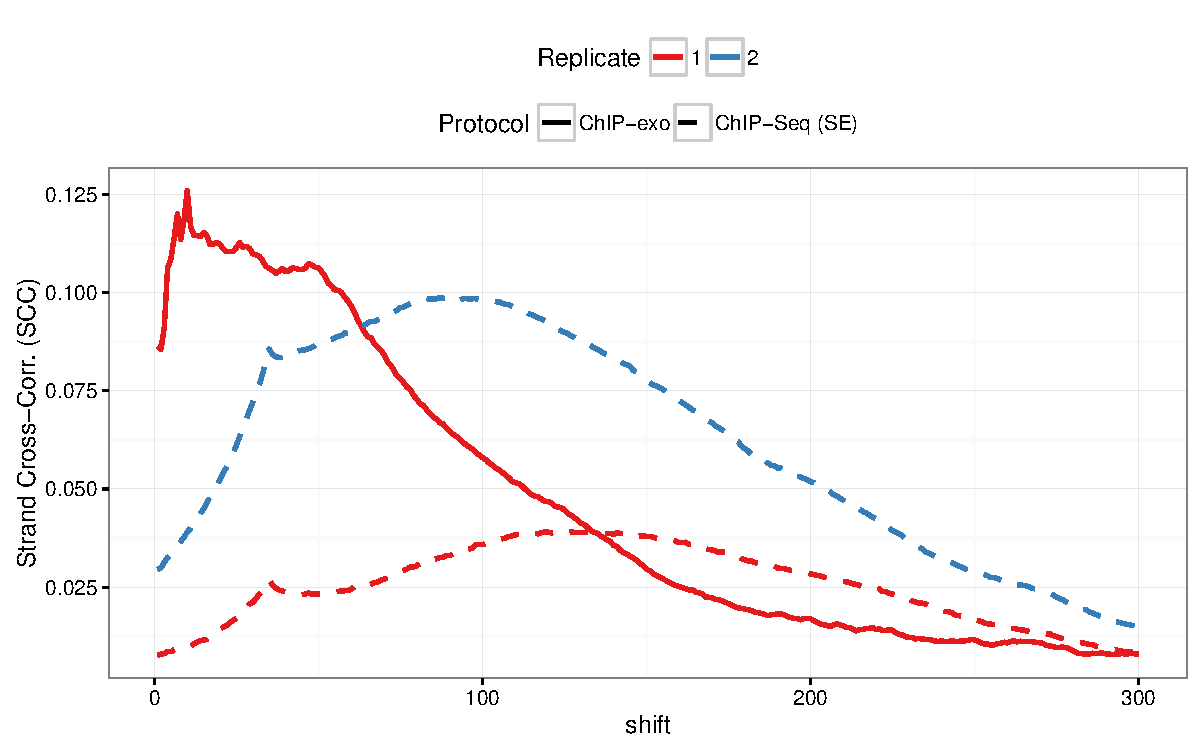
\includegraphics[width = .7\textwidth]{../figs/for_paper/scc_ctcf.pdf}
  \caption{SCC for CTCF factor in HeLa cell line for ChIP-exo (obtained from \cite{exo1}) and SE ChIP-Seq (obtained from \cite{encode1}) }
  \label{fig:scc}
\end{figure}

Figure \ref{fig:scc} shows the SCC function for both a ChIP-exo (in
red) and a SE ChIP-Seq (in green) for CTCF in HeLa cell line. The
ChIP-Seq dataset behaves as the successful case from \cite{encode_qc},
but the ChIP-exo doesn't. Additionally, since the exonuclease enzyme
digests the DNA fragments, then the shifts where the SCC may reach a
local or a global maximum are confounded. Hence, new QC measures are
necessary for ChIP-exo data.

\begin{table}[H]
  \centering
  \caption{Usual quality control indicators applied to the $\sigma^{70}$ samples. PBC stands PCR-bottleneck coefficient (0-0.5 is severe bottlenecking, 0.5-0.8 is moderate bottlenecking, 0.8-0.9 is mild bottlenecking, while 0.9-1.0 is no bottlenecking), NSC for normalized strand cross-correlation coefficient (Another measure related to the strand cross-correlation curve is the RSC was omitted since input sample usually don't exists for ChIP-exo). $\sig$ samples were given by Professor Robert Landick's Lab, FoxA1 and ER samples are from Serandour et al., 2013 \cite{exoillumina} and CTCF sample is from Rhee and Pugh, 2011 \cite{exo1}. }

\begin{tabular}{l|l|r|r|r|r|r}
\hline\hline
IP & Organism  &Condition & Rep. & Nr. reads & PBC &  NSC  \\
\hline\hline
$\sig$ & E.Coli & Rif-0min & 1 & 960,256 & 0.2823 &   10.29 \\
\hline
$\sig$ &  E.Coli & Rif-0min & 2 & 2,247,295 & 0.2656 &  25.08  \\
\hline
$\sig$ &  E.Coli & Rif-20min & 1 & 1,940,387 & 0.2698 &  17.69  \\
\hline
$\sig$ &  E.Coli & Rif-20min & 2 & 4,229,574 & 0.2153 &   14.11 \\
\hline
FoxA1 &  Mouse &  NA & 1 & 22,210,461 & 0.6562 & 21.452 \\
\hline
FoxA1 &  Mouse &  NA & 2 & 22,307,557 & 0.7996 & 60.661 \\
\hline
FoxA1 &  Mouse &  NA & 3 & 22,421,729 & 0.1068 & 72.312 \\
\hline
ER & Human & NA & 1 & 9,289,835 & 0.8082 & 19.843 \\
\hline
ER & Human & NA & 2 & 11,041,833 & 0.8024 & 21.422 \\
\hline
ER & Human & NA & 3 & 12,464,836 & 0.8203 & 19.699 \\
\hline
CTCF & Human & NA & 1 &   48,478,450 & 0.4579 & 15.977 \\
\hline
\end{tabular}  
  \label{tab:qcbase}
\end{table}

\subsection{The dPeak Model}
\label{sec:dpeak}

Chung et al., 2013 proposed the dPeak model to identify the
transcription factor binding sites in high resolution. Two models are
proposed: One to deconvolve the signal of single end reads (SE) data,
i.e. when only one end of the DNA fragment is sequenced; and another
to deconvolve the signal of paired end reads (PE) data, i.e. when both
ends of the DNA fragment are sequenced. For ChIP-exo, only the 5' end
is considered, since is the side where the exonuclease enzyme digests
the DNA.

\newpage

\begin{figure}[H]
  \centering
  \includegraphics[width = .6\textwidth]{/p/keles/ChIPexo/volume3/ChIPexo/poster/dpeak.png}
  \caption{A schematic illustration of dPeak's model when the read is
    located around binding site $\mu_g$}
\end{figure}

Given a peak region with $m$ positions, with $n$ DNA reads and that
the region is generated by a known $g^*$ amount of binding
events. Each read is described by the start position where the 5' end
is aligned and the strand from which the fragment is sequenced. Since
only one end is sequenced, then the fragment length is not
observed. dPeak assumes that the strand $D_i$ follows a Bernoulli
distribution with known parameter $p_D$, the binding event is not
observed and it follows a
$\mbox{Multinomial}(\pi_0,\pi_1,\cdots,\pi_{g^*})$. And the 5' end
$R_i$ for the $i$-th fragment is generated according to the following
procedure:

\begin{itemize}
\item If the read was sequenced from the forward strand ($D_i = 1$):
  \begin{itemize}
  \item The read belongs to the background: $R_i | Z_i = 0, D_i = 1
    \sim \mbox{Unif}(1, m)$
  \item The read belong to the $g$-th binding event: $R_i | Z_i = g,
    D_i = 1 \sim \mbox{N}(\mu_g - \delta , \sigma^2)$
  \end{itemize}
\item If the read was sequenced from the backward strand ($D_i =
  0$):
  \begin{itemize}
  \item The read belongs to the background: $R_i | Z_i = 0, D_i = 1
    \sim \mbox{Unif}(1 , m)$
  \item The read belong to the $g$-th binding event: $R_i | Z_i = g,
    D_i = 1 \sim \mbox{N}(\mu_g + \delta , \sigma^2)$
  \end{itemize}
  
\end{itemize}

\subsubsection{A New Initialization Strategy for dPeak}
\label{sec:algo}

dPeak's model likelihood is optimized by the stochastic EM
algorithm. Hence, it is of utmost importance how the parameters are
initialized in order to obtain a global maximum.

Chung et al., 2013 \cite{dpeak} derived an initialization strategy for
the stochastic EM algorithm where for each region, the binding sites
locations $\mu_g, g=1,\cdots,g^*$ were initialized equally spaced
around the region and the parameters $\delta$ and $\sigma$ were
estimated by separate for all regions. This is problematic since this
initialization strategy does not depend on the data, specially in
regions with low signal to noise ration and with a low amount of
reads.

For this work, we considered a new strategy where the $mu_g$'s are
initialized by partitioning the region into $g^*$ bins and finding the
coverage's local maxima in each bin and we initialize $\delta$ and
$\sigma$ by ranking the regions by the signal strength or an empirical
quantity (as the number of ChIP tag counts in the region), fit the
model for the top $N_{\text{top}}$ regions and then use as initial
values the average of the $\sigma$ and $\delta$ estimates for those
regions.

\subsection{Comparison with ChIP-Seq data}
\label{sec:comp_chipseq}



We first compared various factors that could affect binding site
identification between ChIP-exo and ChIP-Seq data. In order to compare
distribution of signal and background between ChIP-exo and ChIP-Seq
data, we calculated ChIP tag counts across the genome by counting the
number of reads mapping to each of 150 non-overlapping
window after extending reads by 150 to their 3' end
directions. ChIP tag counts in ChIP-exo data were linearly related to
ChIP tag counts in ChIP-Seq data for the regions with high ChIP tag
counts (Figure \ref{fig:comp}A). This implies that signals for
potential binding sites are well reproducible between ChIP-exo and
ChIP-Seq data. On the other hand, there was clear difference in the
background distribution between them. In ChIP-Seq data reads were
almost uniformly distributed over background (non-binding) regions and
the ChIP tag counts in there regions were significantly larger than
zero. In contrast, in ChIP-exo data, there was larger variation in
ChIP tag counts among background regions and ChIP tag counts were much
lower in these regions compared to ChIP-Seq data. There were also
large proportion of regions without any read in ChIP-exo data. These
results indicate that for ChIP-exo data a much smaller portion of the
genome is expected to be background.

\begin{figure}[H]
  \centering
  \includegraphics[width = .46\textwidth,page = 3 ]{../figs/for_paper/ChIPseqPET_ChIPexo_tagCount_comparison.pdf}
  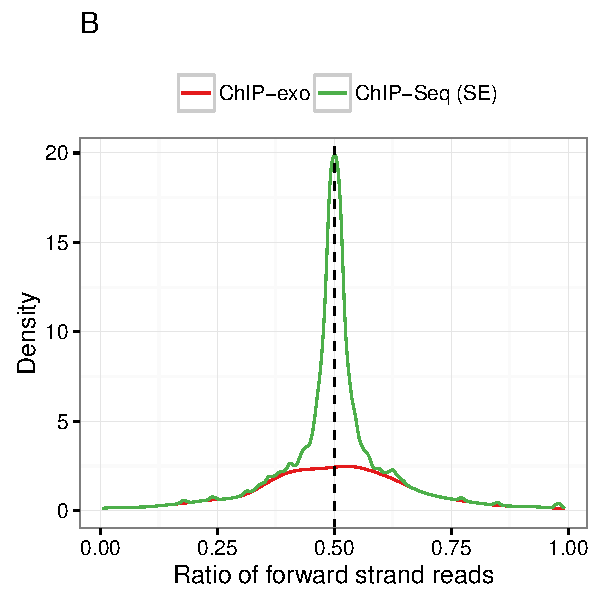
\includegraphics[width = .46\textwidth]{../figs/for_paper/forward_strand_ratio_comp_old.pdf}
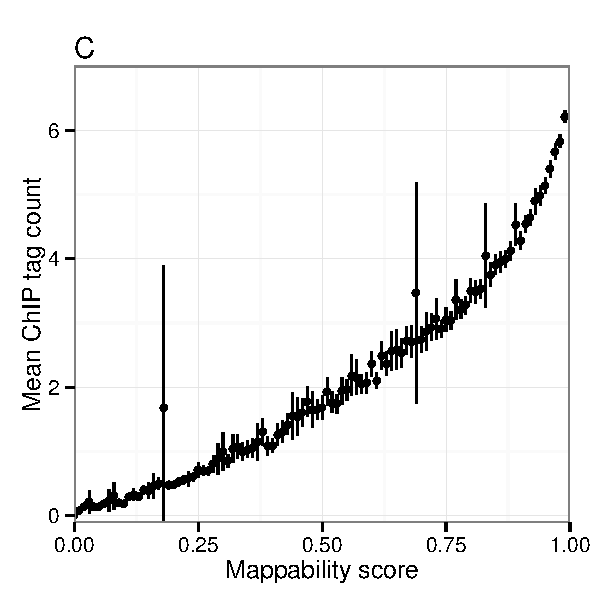
\includegraphics[width = .46\textwidth,page = 1]{../figs/for_paper/eukaryotic_bias_CTCF.pdf}
  \includegraphics[width = .46\textwidth,page = 2]{../figs/for_paper/eukaryotic_bias_CTCF.pdf}
  \caption{ A) Hexbin plot of PE ChIP-Seq bin counts VS ChIP-exo bin
    counts. B) Forward Strand Ratio densities for SE ChIP-Seq and
    ChIP-exo peaks. C) ChIP tag counts increase linearly as
    mappability scores increases. D) ChIP tag counts increase linearly
    as GC content score increases when GC content is less than 0.6 and
    then ChIP tag counts decrease as GC content increases. }
  \label{fig:comp}
\end{figure}

We next evaluated the ``peak pair'' assumption from Rhee and Pugh,
2011 \cite{exo1}, i.e. a peak of reads in the forward strand is
usually paired with a peak of reads in the reverse strand that is
located in the other site of the binding site. Wang et al., 2014
\cite{mace}, Madrigal 2015 \cite{cexor} and Bardet et al., 2013
\cite{peakzilla} proposed method rely in this assumption. In order to
evaluate this assumption, we reviewed the proportion of reads in the
forward strand in candidate regions (i.e. regions with at least one
binding site) in $\sig$ ChIP-exo data. We found that strands of reads
were much less balanced in ChIP-exo data than in ChIP-Seq data in
these regions with potential binding sites (Fig. \ref{fig:comp}B) and
this indicates that the peak pair assumption might not hold in real
ChIP-exo data.

We evaluated ChIP-exo data for CTCF factor from human genome
\cite{exo1} to investigate issues specific to eukaryotic genomes for
binding sites identification. Figures \ref{fig:comp}C and
\ref{fig:comp}D display the bin-level average read counts against
mappability and GC content. Each data point is obtained by averaging
the read counts across bins with the same mappability of GC
content. These results indicate that binding site identification in
ChIP-exo sample might also benefit from the use of methods that take
into account of apparent sequence biases such as mappability and GC
content.

\section{Results}
\label{sec:results}

\subsection{ChIP-exo Quality Control Pipeline}
\label{sec:QC}

Figure \ref{fig:qcdiagram} shows a flowchart for the ChIPexoQC
pipeline. Which basically partitions the genome by keeping the
non-digested ChIP-exo regions. Then, for each region it calculates a
series of statistics. Finally, it creates several visualizations
designed to assess the quality levels of a ChIP-exo sample.

\begin{figure}[h!]
  \centering
  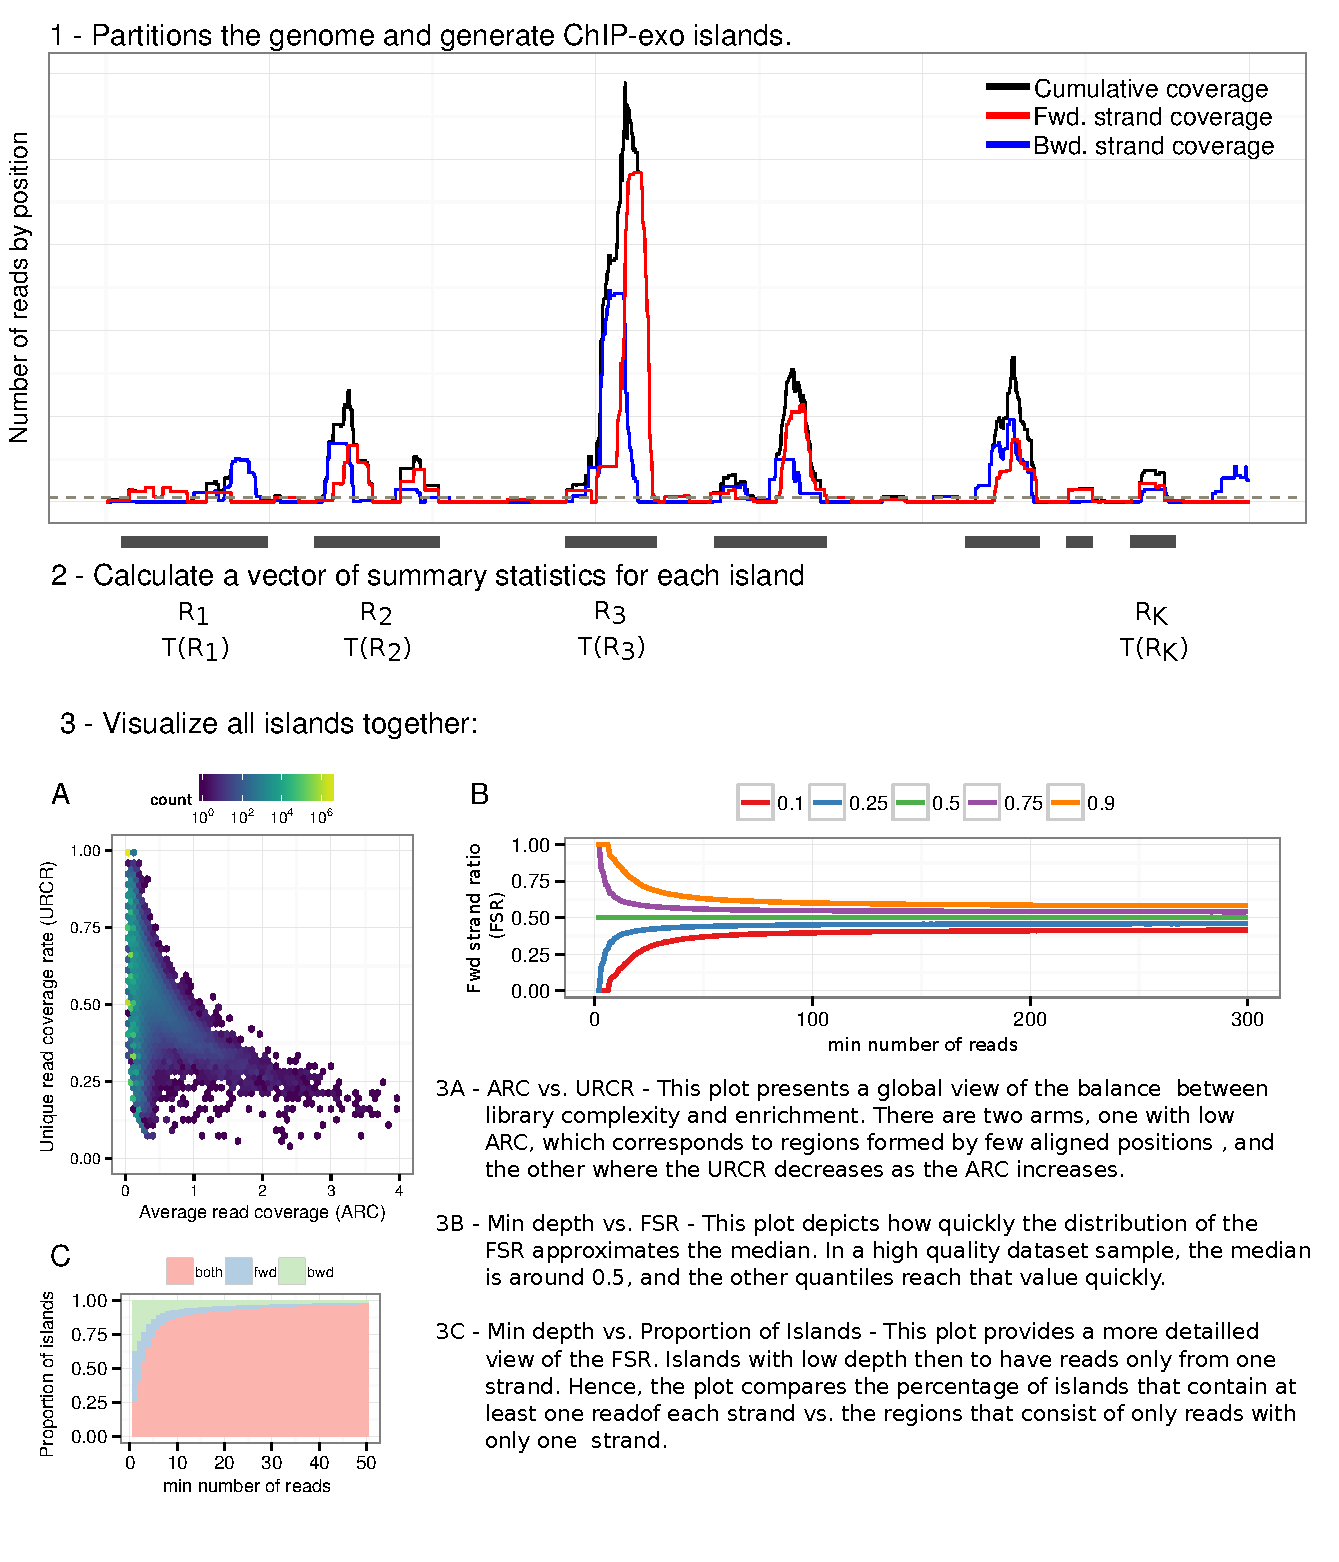
\includegraphics[width = .7\textwidth]{../figs/for_paper/coverage_diagram2.pdf}
  \caption{Flowchart of the ChIP-exo Quality control pipeline.}
  % The genome is partitioned into several regions by removing the empty
  % segments and for each regions we calculate a collection of QC
  % indicators, then for each region $R_k$ a vector of summary
  % statistics $T(R_k)$ is calculated.
  \label{fig:qcdiagram}
\end{figure}

\subsubsection{Normalized Local Strand Cross-Correlation}
\label{sec:locNSC}

We considered the creation of a novel QC measure for ChIP-exo called
local normalized SCC or $\mbox{local-NSC}$. This measure is built by
calculating the SCC for a given region:

\begin{align}
  y(\delta) = r\left[ n^+ \left(x + \frac{\delta}{2}
    \right), n^- \left( x- \frac{\delta}{2} \right)\right]
\nonumber
\end{align}

where again $r$ is the Pearson correlation but $n^+$ and $n^-$ are the
coverage vectors of a given region in the genome. Figure
\ref{fig:locSCC} shows that as the library complexity of the region is
lower, then the local SCC seems to show higher variance. Hence, we
fit a nonparametric regression model to smooth the SCC signal:

\begin{align}
 y(\delta) &= f(x_\delta) + \epsilon_\delta \nonumber
\end{align}

where $y(\delta)$ is the observed SCC for shift $x_\delta$,
$\epsilon_\delta \sim N(0,\sigma_f^2)$. 


Finally the $\mbox{local-NSC}$ is defined as:

\begin{align}
    \mbox{local-NSC} &= \frac{\mbox{max}_{x_\delta} \hat{f}(x_\delta)}{\hat{\sigma}_f} 
\label{locNSC}
\end{align}

Local NSC gives a signal-to-noise ratio for a given region in a
ChIP-exo sample. 

\begin{figure}[H]
  \centering
  \includegraphics[width = .9\textwidth]{../figs/for_paper/local_SCC_example.pdf}
  \caption{Using the FoxA1 sample from \cite{exoillumina}. A) shows an
    example region for the 3 replicates. The library complexity seem
    to be comparable between the two top rows and both outperform the
    last row. The number of reads for the first replicate is higher
    than the number of reads for the other replicates. B) Shows the
    local SCC for the 3 replicates, this measure is comparable among
    the 3 replicates. The first replicate shows the lowest residual
    error, while the third one shows the highest. In blue, a ``loess''
    regression model is fitted.}
\label{fig:locSCC}
\end{figure}

\subsubsection{Enrichment and Library Complexity in ChIP-exo data}
\label{sec:enri}

In ChIP-exo experiments, the background is often digested by the
exonuclease enzyme, therefore to determine the sample's quality is
necessary to address the balance between the enrichment and library
complexity. To diagnose this, we consider the Average Read Coverage
(ARC) and the Unique Read Coverage Rate (URCR) which are defined as:

\begin{align}
  \mbox{ARC} &= \frac{\text{Nr. of reads in the region}}{\text{Width of the region}} \nonumber \\
  \mbox{URCR} &= \frac{\text{Nr. of reads mapped to only one position
      in the region}}{\text{Nr. of reads in the region}} \nonumber
\end{align}

Figure \ref{fig:enrich}A shows hexbin plots illustrating the
relationship between library complexity and sample enrichment for the
FoxA1 in mouse cells from \cite{exoillumina}. Notice how there are two
strong arms in each panel: The first one corresponds to regions with
low $\mbox{ARC}$ values and varying $\mbox{URCR}$ values across the
$(0,1]$ interval, while the second one shows a decreasing trend in
$\mbox{URCR}$ as $\mbox{ARC}$ increases. When an experiment shows a
higher degree of enrichment, then the separation of this two arms is
more noticeable, since as Figures \ref{fig:enrich2}A and
\ref{fig:enrich2}B show the ARC VS URCR plots but filtering out the
regions formed by a low number of unique positions (10 and 30
respectively), hence this second arm corresponds to possibly enriched
regions.



Figure \ref{fig:enrich}B shows box plots of the $\mbox{local-NSC}$ on
regions of the three replicates, stratified by the number of reads
mapped exactly to one position for all Fox-A1 ChIP-exo experiments;
The high stratum is defined by regions consisting of more than
100 unique positions, the medium stratum for regions where
the number of unique position is on the (50,100)
range and the low stratum in the (20,50) range. For
each stratum and biological replicate, we sampled 400
regions whenever possible (in the opposite case, all the regions in
the category were considered) and calculated the $\mbox{local-NSC}$
for those regions. On one side, we can see that for all three
replicates, as the number of unique positions increases, then the
$\mbox{local-NSC}$ shows higher values. In the low panel, all three
replicates are comparable, in the medium panel, the first two
replicates are comparable and both outperform the third one, and
finally in the high panel we can see that despite that the first two
replicates are comparable, the first one slightly outperforms the
second. We can see that all three panels coincide with the conclusion
we get from Figure \ref{fig:enrich}A: First, the first replicate seems
to have the highest library complexity and the third replicate the
lowest. Second, despite that both first two replicates show a similar
level of bottlenecking, the regions in the first replicate seems to
have a higher ARC, those regions seem to be contributing to have a
higher local-NSC in the high panel. Third, despite that the ARC of the
first and third replicates is comparable, the third replicate has a
higher bottlenecking level which cause to $\mbox{local-NSC}$ to have
lower levels overall.

\begin{figure}[H]
  \centering
  \includegraphics[width = .7\textwidth]{../figs/Carroll_mice_for_paper/FoxA1_enrichment.pdf}
  \includegraphics[width = .7\textwidth,page =4]{../figs/Carroll_mice_for_paper/Local_SCC_indicator_by_strata.pdf}
%  \includegraphics[width = .7\textwidth,page =4]{../figs/Carroll_mice_for_paper/Local_SCC_indicator_by_strata_sameRegion.pdf}
  \caption{Using the mouse-FoxA1 experiment from \cite{exoillumina}:
    A) Hexbin plots of $\mbox{ARC}$ against $\mbox{URCR}$, in general
    we can see a slight separation into two strong arms, one
    corresponds to low $\mbox{ARC}$ and varying $\mbox{URCR}$, and for
    the other $\mbox{URCR}$ decreases as $\mbox{ARC}$ increases B)
    Boxplots of the $\mbox{local-NSC}$ stratified by nr. of reads
    mapped to only one position in the regions for the ChIP-exo
    experiments divided by condition and biological replicate.}
  \label{fig:enrich}
\end{figure}


% and C) Boxplots of the a set of the first replicate regions,
% stratified as in (B) with the $\mbox{local-NSC}$ calculated with the
% different biological replicates.

\subsubsection{Strand Imbalance in ChIP-exo data}
\label{sec:strand_imbalance}

The strand imbalance assessment is based in the observation that the
enriched regions usually have a higher concentration of reads,
therefore we examined the FSR (defined as the ratio of the number of
forward stranded reads divided by the total number of reads in a given
region) as the region with lower depth are being filtered out. This
indicator is of particular importance, since several methods rely on
the ``peak-pair'' assumption. In Table \ref{tab:qcbase}, we calculated
the FSR and noticed that for all the samples, it's value is close to
0.5, which means that there are roughly the same amount of reads in
both strands. However, Figure \ref{fig:comp}B shows that this value
doesn't represent the sample locally, hence the assumption doesn't
hold well in practice.



In order to assess the strand imbalance we created the following
visualization presented in Figure \ref{fig:strand}. A) shows the FSR's
behavior as lower depth regions are being filtered out, while B) shows
which percentage of the regions are composed by reads of both strands
or only one (forward or backward). As the number of reads per region's
lower bound increases, the quantiles tend to approach the median. To
evaluate this statement, for each replicate of FoxA1, we divided the
regions formed by at least 100 reads into the ones that overlap
with any of the sample's peaks. Then we considered Kolmogorov-Smirnov
tests to assess if the FSR's distribution was the same for the islands
that overlap with a peak and the islands that didn't. The p.value for
the third replicate's test is 0.1039, for the first
replicate's test is 0.0064 and for the second test is
0.0871. This shows that only the middle sample from Figure
\ref{fig:strand} is the least imbalance sample from the the three,
while the other two still show a higher imbalance at the 100
level.

\begin{figure}[H]
  \centering  
  \includegraphics[width = .8\textwidth,page = 3]{../figs/Carroll_mice_for_paper/Strand_imbalance.pdf} 
  \caption{Strand imbalance QC plots for the same data as in Figure
    \ref{fig:enrich}. A) FSR distribution quantiles as the lower depth
    regions are being filtered out, all quantiles approach to the
    median as the lower bound increases. B) Stacked histogram with the
    proportion of regions that are formed by two strands or only one,
    in a good sample the single-stranded regions are going to be
    filtered out quickly as in the middle row.}
  \label{fig:strand}
\end{figure}

\subsection{Comparison with ChIP-Seq data using dPeak}
\label{sec:dpeak_analysis}




Figure \ref{fig:reso_all} shows different comparisons among ChIP-exo,
PE ChIP-Seq and SE ChIP-Seq. A RegulonDB annotation was considered
identified if the distance between it and dPeak binding site estimate
was at most of 20 bp. That way, the sensitivity is defined as
the proportion of RegulonDB annotations identified in a peak (Salgado
et al., 2012 \cite{regulonDB}). Figure \ref{fig:reso_all}A illustrates
that the sensitivity of all protocols increases as the average
distance between binding sites does. Despite that when the binding
events in a peak are closer to each other, both ChIP-exo and PE
ChIP-Seq are comparable, as the distance increases ChIP-exo identifies
a higher proportion of the RegulonDB annotations; additionally SE
ChIP-Seq is significantly less sensitive than both ChIP-exo and PE
ChIP-Seq. In Figure \ref{fig:reso_all}B the distance between a
RegulonDB annotation to its closest prediction is compared for
ChIP-exo, PE and SE ChIP-Seq; while the first two are comparable,
both outperform SE ChIP-Seq.

In Figures \ref{fig:reso_all}C and \ref{fig:reso_all}D, we observe the
behavior of dPeak's estimated parameters for single end data (both
ChIP-exo and ChIP-Seq). The $\delta$ parameter measures the distance
from the 5' end of the read's 5' end to its respective binding event
and the $\sigma$ parameter indicates the read's starting position
distribution variability around their respective binding sites (more
information in \cite{dpeak}). For both parameters, it can be seen that
the ChIP-exo estimates are smaller than the SE ChIP-Seq estimates in
average, which agrees with the fact that the sample reads are
allocated more tightly around the binding events in ChIP-exo
data. This confirms that the dPeak model is able to recover the same
conclusions that have been done when comparing ChIP-exo and SE
ChIP-Seq.

% Hence we can conclude that the peaks shape is quite different
% between ChIP-exo and SE ChIP-Seq.
\begin{figure}[H]
  \centering
  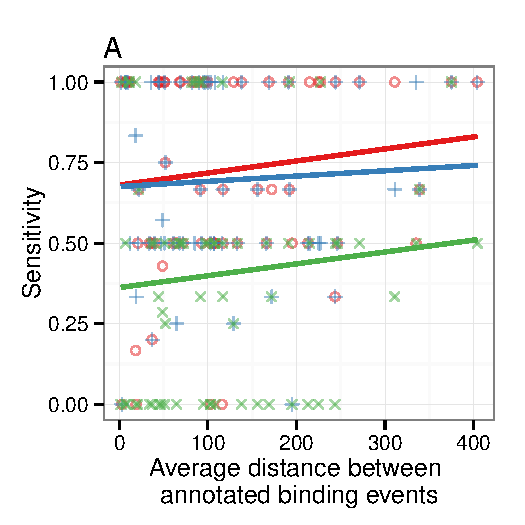
\includegraphics[width = .46\textwidth]{../figs/for_paper/sensitivity_exo_olda_data.pdf}
  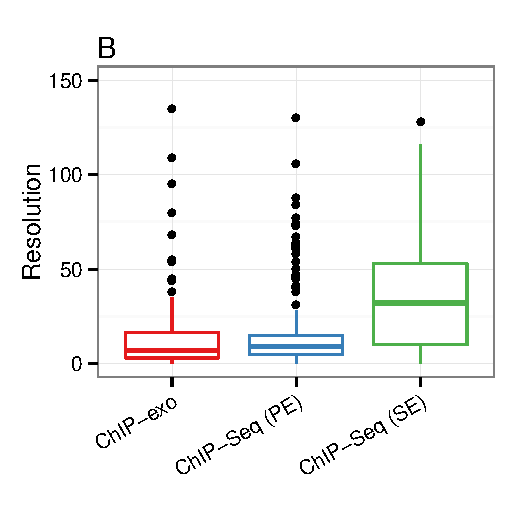
\includegraphics[width = .46\textwidth]{../figs/for_paper/resolution_by_dataset_old_data.pdf}
\end{figure}

\begin{figure}[H]
\centering
   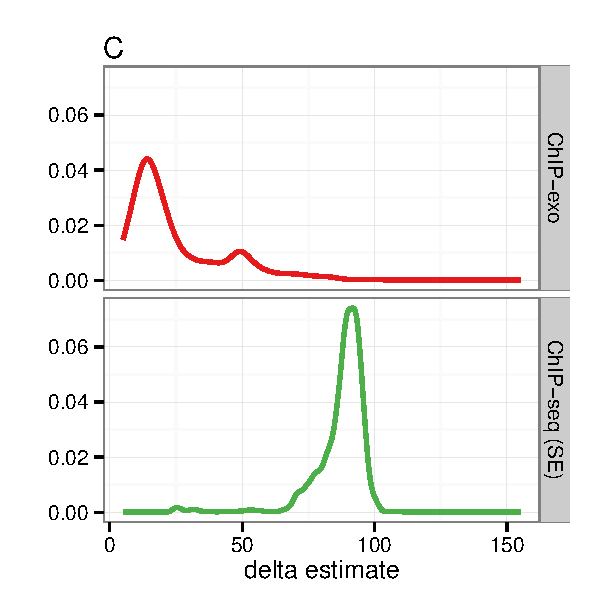
\includegraphics[width = .46\textwidth,page = 1]{../figs/for_paper/sigma_delta_old_densities.pdf}
   \includegraphics[width = .46\textwidth,page = 2]{../figs/for_paper/sigma_delta_old_densities.pdf} 

   \caption{Comparison of (A) sensitivity and (B) resolution between
     ChIP-exo and ChIP-Seq data. Sensitivity is defined as the
     proportion of RegulonDB annotations identified using each
     data. Resolution is defined as the distance between RegulonDB
     annotation and its closest prediction. $\quad$ C) $\delta$ parameter in
     dPeak measures average distance of the reads to their respective
     binding site. In ChIP-exo data, reads were located much closer to
     the binding site than in SE ChIP-Seq. D) $\sigma$ parameter
     measure the dispersion of reads around each binding site. In
     ChIP-exo data, reads showed less variation around the their
     respective binding sites compared to SE ChIP-Seq.}
  \label{fig:reso_all}
\end{figure}

\subsection{Systematic Comparison of ChIP-Seq vs ChIP-exo under
  Varying Sequencing Depths}
\label{sec:reco}



Previously, ChIP-exo and SE ChIP-Seq have been compared at a fixed
depth level in the literature, but this comparisons didn't included PE
ChIP-Seq. Hence, we sampled a fixed amount of reads for each of the
ChIP-exo, PE ChIP-Seq and SE ChIP-Seq datasets of the $\sigma^{70}$
sample in aerobic conditions. For each sampled dataset we applied our
lower-to-higher resolution pipeline by calling peaks with MOSAiCS
\cite{mosaics} and then deconvolving the binding events by using dPeak
\cite{dpeak}. For the ChIP-exo datasets we called peaks by using
GC-content and mappability with MOSAiCS, and for the ChIP-Seq datasets
we used their respective Input samples.

\begin{figure}[H]
  \centering
%  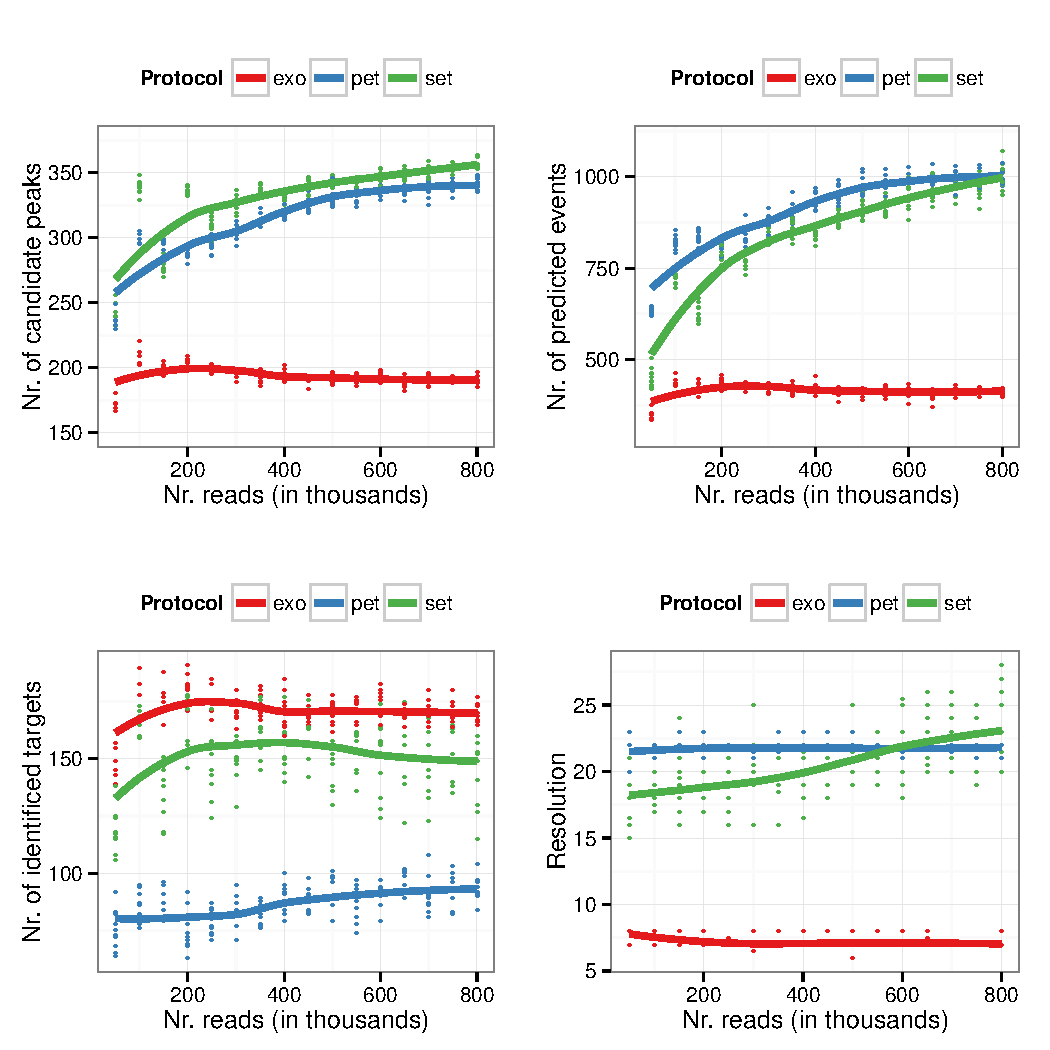
\includegraphics[width = .8\textwidth]{../figs/for_paper/Sig70_aerobic_saturation.pdf}
  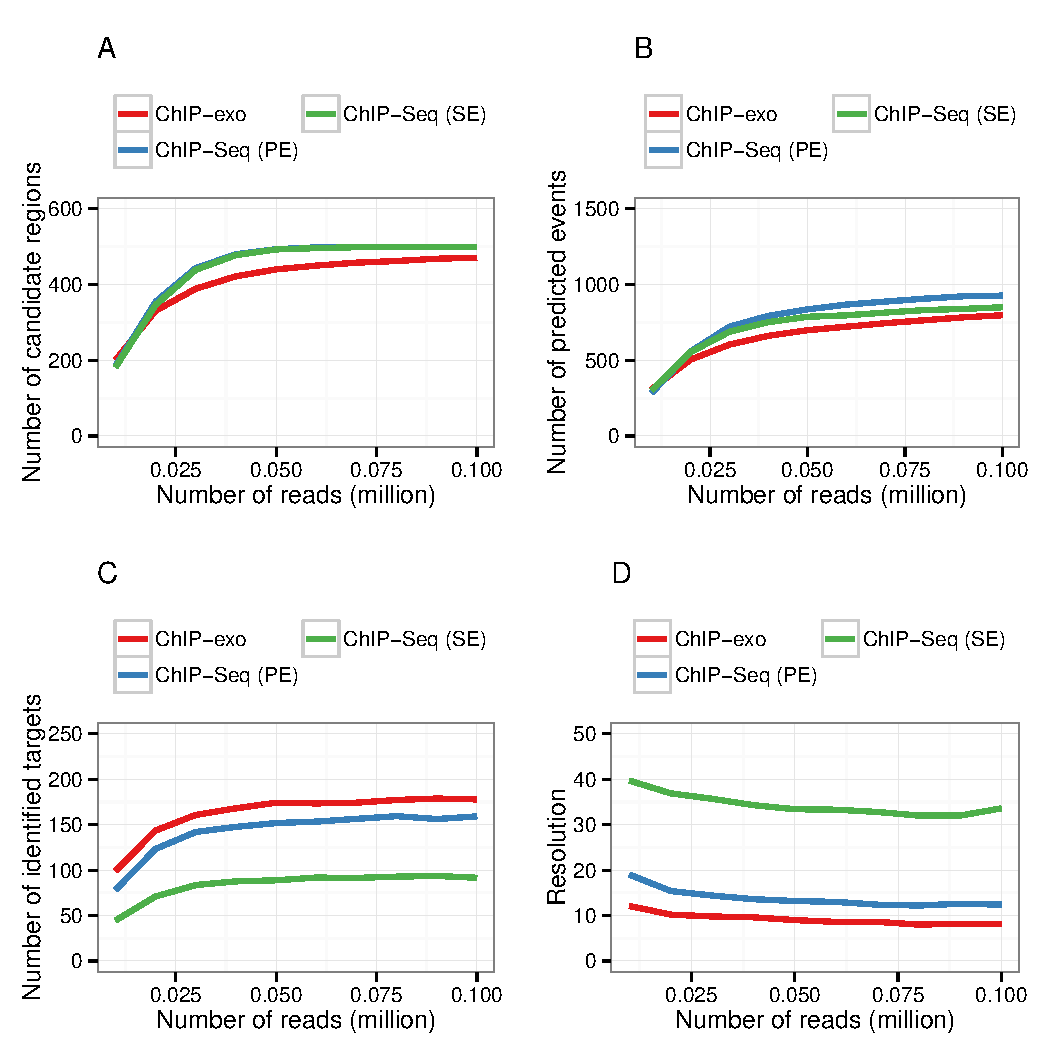
\includegraphics[width = .8\textwidth]{../figs/for_paper/saturation_analysis_old.pdf}
  \caption{\textbf{ChIP-exo, PE ChIP-Seq and SE ChIP-Seq comparison at
      varying sequencing depths}Comparison of the number of candidate
    regions (A), predicted events (B), identified targets (C) and
    resolution (D) among ChIP-exo, PE ChIP-Seq and SE
    ChIP-Seq. RegulonDB annotations are considered as a gold
    standard. A gold standard binding events was deemed identified if
    a binding event was estimated at a $\pm$ 15 vicinity of
    it.}
  \label{fig:design}
\end{figure}

Figure \ref{fig:design} shows the behavior of each data type when
their depth is fixed. It is remarkable that even when the number of
candidate peaks or the number of predicted events is lower for
ChIP-exo, it outperforms both PE and SE ChIP-Seq in the number of
identified targets and resolution. This may suggest that with ChIP-exo
less false positive peaks are being called and that when the targets
are being identified, dPeak estimates binding locations closer to the
true location. Additionally, we can see that as the read depth
increases all four indicators do so as well, which may indicate that
with ChIP-exo a smaller amount of reads is necessary to identify a
higher number of targets, but it may also be possible that this is an
artifact occurring due to ChIP-exo's lower library
complexity. Additionally, it is worth noting that for PE ChIP we
sampled both ends of the fragment, hence for each sequencing depth
considered we are sampling twice as many reads for PE ChIP-Seq than
for ChIP-exo or SE ChIP-seq.

\section{Software packages}
\label{sec:software}

For this project several R packages were created or updated:

\begin{itemize}
\item \textbf{dPeak}: We updated the initialization strategy. The
  latest version is currently available from
  \url{http://dongjunchung.github.io/dpeak/}.
\item \textbf{ChIPexoQual}: This package contains the QC pipeline for
  ChIP-exo. The last version is available in
  \url{https://github.com/welch16/ChIPexoQual}.
\item \textbf{Segvis}: The goal of this package is to visualize
  genomic regions by using aligned reads such as in Figures
  \ref{fig:exo} or \ref{fig:qcdiagram}.  The latest version is
  available in \url{https://github.com/keleslab/Segvis}.
\item \textbf{ChIPUtils}: This package attempts to gather the most
  commonly used ChIP-Seq QC (as in Table \ref{tab:qcbase} or Figure
  \ref{fig:scc}) indicators and additional utilities (as Figure
  \ref{fig:comp}A) for ChIP-Seq. The latest available version is in
  \url{https://github.com/welch16/ChIPUtils}.
\end{itemize}

\section{Conclusions}
\label{sec:conclusions}

We provide a ChIP-exo QC pipeline capable of assess the balance
between enriched samples and low complexity regions. It is shown that
the ``peak-pair'' assumption doesn't hold locally in practice and we
provide two out-of-the-box visualization capable to assess the strand
imbalance in a ChIP-exo experiment.

We showed that ChIP-exo is comparable in resolution with PE ChIP-Seq
and both outperforms SE ChIP-Seq. ChIP-exo shows higher sensitivity
than ChIP-Seq (both PE and SET), and this effect increases when the
average distance between binding events is larger.

We demonstrated for the first time that when ChIP-exo is compared with
PE ChIP-Seq (and SE ChIP-Seq) at a fixed sequencing depth, ChIP-exo is
able to identify more targets at a lower resolution. dPeak provides a
striking balance in sensitivity, specificity and spatial resolution
for ChIP-exo analysis.


% We compared dPeak with another
% algorithms to estimate binding locations in ChIP-exo data, dPeak is
% comparable to MACE and outperforms GEM in resolution. dPeak provided a
% striking balance in sensitivity, specificity and spatial resolution
% for ChIP-exo analysis.


\newpage


\section{Planned work}
\label{sec:future}

\subsection{Additional Thoughts for this Analysis}

\subsubsection{GC Content and Mappability Quality Indicators}
\label{sec:gc_map_qc}

Figure \ref{fig:comp} shows a relationship between the ChIP tag counts
of a ChIP-exo experiment and both mappability and GC content
scores. Furthermore, in sections \ref{sec:reco} and
\ref{sec:dpeak_analysis} we called peaks by using MOSAiCS which
considers them as necessary information when there is not control (the
GOF plot is in Figure \ref{fig:mosaics_exo}) sample. Hence, we may add
QC measures that consider the GC content and mappability score biases
into the QC pipeline.

\subsubsection{Quality Control for ChIP-Nexus}
\label{sec:nexus}

% For example, the recently described ChIP-nexus protocol ligates both
% sequencing adaptors onto one end of ChIP fragments in a single step
% (as opposed to two separate ligation steps in the original ChIP-exo
% protocol) (He et al., 2015). Exonuclease digestion, DNA
% self-circularization with circLigase, and restriction enzyme cutting
% between the two adaptors creates the final library. By removing one
% of the relatively inefficient ligation steps, ChIP-nexus yields
% higher complexity libraries with the same resolution as
% ChIP-exo. One concern is that circLigase activity might have
% sequence specificity (Kwok et al., 2013), potentially creating bias
% in the identification of binding locations.

He et al., 2014 \cite{chipnexus} proposed a modification to the
ChIP-exo protocol that may fix its low library complexity issues by
extending the reads by a random barcode prior to the exonuclease
digestion and ligating both sequencing adaptors onto one end of the
ChIP DNA fragment (as opposed to two separate ligation steps in
ChIP-exo). We want to apply our QC pipeline to ChIP-Nexus. Depending
on the depth of the regions formed by ChIP-Nexus data, we may need to
modify the QC pipeline in the step where it partitions the reads into
regions, but the $\mbox{local-NSC}$ may be used to prove this
statement.

\subsection{Analysis of \emph{E. Coli} Transcription Initiation Complexes}
\label{sec:ecoli}

The data showed in Figure \ref{fig:exo_example} is actually part of a
more interesting experiment from Professor Landick's lab. We have 2
biological replicates of the $\sig$, $\beta'_f$ and $\beta$
transcription factors under two conditions, one where rifampicin was
applied by 20 minutes and another where it wasn't applied. As seen in
the Figure, there is ChIP-exo data for the 3 factors and PE ChIP-Seq
for $\sig$ and $\beta'_f$ (in the Figure both replicates were pooled).

$\sig$ factor is a transcription initiation factor of housekeeping
genes in \emph{E. Coli}, and both $\beta$ factors transcribe the DNA into
mRNA. Hence, we want to use this data to have a better understanding
of the transcription in \emph{E. Coli}.

The steps in formation of productive transcription complexes are:

\begin{enumerate}
\item Binding of RNAP to promoter DNA to form a closed complex.
\item Rearrangement of RNAP-DNA contacts to form an open complex.
\item Binding of nucleotide triphosphates in the active site and
  synthesis of a initial RNA to yield an initial transcription complex
  (ITC) - this is sometimes called a ``scrunched complex''.
\item Promoter escape to form a elongated complex (EC$_1$) when the
  promoter contacts are broken, and the $\sig$ factor is released.
\item Conversion of EC$_1$ into EC$_2$ by loading of the ribosome and
  elongation factors to enable efficient transcript elongation.
\end{enumerate}

% \begin{figure}[H]
% \centering
% \begin{tikzpicture}[node distance = 3cm]
% \tikzstyle{region} = [draw,thin,fill = blue!20]
% \tikzstyle{line} = [draw,thick]
% %\path[use as bounding box] (-1,0) rectangle (10,-2);
% \path[-] node[region] (step1) {RNAP + Promoters};
% \path[-] node[region,right of =step1,fill = red!20] (step2) {Closed};
% \path[-] node[region,right of =step2,fill = green!20] (step3) {Intermediate};
% \path[-] node[region,right of =step3,fill = yellow!20] (step4) {Open};
% \path[line][<->] (step1) -- (step2);
% \path[line][<->] (step2) -- (step3);
% \path[line][<->] (step3) -- (step4);
% \end{tikzpicture}
% \caption{Zooming into transcription}
% \end{figure}

As a proof of concept we were able to identify open and closed regions
by centering the binding the peaks respect to the highest $\sig$
summit (among the rif0 and rif20 samples), and then using hierarchical
clustering on the $\beta'_f$ signal of the rif0 samples to produce:

\begin{figure}[H]
  \centering
 \includegraphics[width = \textwidth]{/p/keles/ChIPexo/volume5/OpenClosedComplexes/figs/filtered/heatmaps_centroid.png}
 \caption{Centered and normalized heatmaps for PE ChIP-Seq peaks of
   $\sig$ and $\beta'_f$ under rif0 and rif20. The regions are
   organized by the centroids clustering of the $\beta'_f$-rif0
   profiles.}
  \label{fig:hm1}
\end{figure}

Figure \ref{fig:hm1} shows heatmaps of the normalized coverages of PE
ChIP-Seq peaks for $\beta'_f$ and $\sig70$ under rif0 and rif20
treatments. Each row represents the same region, under the four
different samples. As expected the signal for both $\sig$ samples is
centered around the middle, for $\beta'_f$-rif20, the majority of the
signal seems to be centered, hence the transcription was interrupted
and for $\beta'_f$-rif0 we can see clusters formed by open regions.

Then, using a set of high quality PE ChIP-Seq peaks and clustering
with the mclust model by Fraley and Raftery, 2007 \cite{mclust} we
were able to label the a set of regions as closed or open
complexes. Hence, we expect that by using ChIP-exo data we may find
different patterns that represent transcription units whose output was
limited at different steps in the formation of EC$_2$.

Additionally if we find several cases of those patterns, then we may
be able to determine which sequences may be causing this behavior at
the different steps.

\subsection{Enhancer Prediction and Active Learning}
\label{sec:enhancer}

Last summer, we entered to a contest from ENCODE's functional
characterization group to fit a model to classify enhancers. Roughly
speaking, the dataset consisted of a set of regions
$\mathcal{R}_1,\cdots,\mathcal{R}_n$ and a set of labels
$Y_1,\cdots,Y_n \in \{0,1,\}$. Hence, we built a series of features
$X_1,\cdots,X_p$ and fitted a model. The model was trained by using
10-fold CV and we selected the tunned parameters that maximized the
area under the ROC curve. Then, an independent test set was provided
for which we delivered a set of predictions. However, there are in
total another $m >> n$ regions in the experiment, and the cost of
labeling those $m$ regions may be high (in either the actual monetary
cost of the experiment or the time the scientists spends labeling
those regions). Those $n+m$ regions are H3K27ac peaks, hence they were
ranked and the first $n$ were selected randomly from groups with high,
medium and low signal. This raises the following questions:



\begin{itemize}
\item Is there a better way of ranking these $n+m$ regions ?
\item What is the best way to select the regions that are going to be
  labeled, i.e. we would want to label the region that gives the
  best model fit.
\end{itemize}

Hence, it may be worth to investigate which active learning strategies
may be the best to apply in this particular problem. Settles, 2012
\cite{al} is a survey of active learning techniques that we want to
explore in order to solve these problems.

\newpage

\bibliographystyle{plain} % Style BST file (bmc-mathphys, vancouver, spbasic).
\bibliography{chip_exo_paper}
\nocite{exo_review}
\nocite{exo_gb}
\nocite{maplot1}
\nocite{maplot2}
\nocite{esl}
\nocite{anp}
\nocite{al}
\nocite{oc_review}
\nocite{exo4}

\newpage

\section*{Supplementary materials}
\label{sec:supp}

\subsection*{Additional Enrichment Plots for FoxA1}
\label{sec:enrichsup}

In Figure \ref{fig:enrich2} it is shown the same relationship as in
Figure \ref{fig:enrich}, but considering only regions formed where the
reads are being allocated in more than 10 (A) and 30 (B) unique
positions respectively. Both plots show that the vertical arms formed
by regions with low $\mbox{ARC}$ is formed by low complexity regions,
that way suggesting that this segment correspond to the background of
a ChIP-exo experiment.

\begin{figure}[h!]
  \centering
  \includegraphics[width = .8\textwidth,page = 3]{../figs/Carroll_mice_for_paper/FoxA1_enrichment.pdf}
  \includegraphics[width = .8\textwidth,page = 4]{../figs/Carroll_mice_for_paper/FoxA1_enrichment.pdf}
  \caption{Hexbin plots of $\mbox{ARC}$ vs $\mbox{URCR}$ for each
    region after partitioning the genome. In A and B the regions with
    reads mapped to at most 10 and 30 positions respectively where not
    considered. $\mbox{ARC}$ is defined as the ratio of the nr. of
    reads and the width of a region and $\mbox{URCR}$ is the ratio of
    the number of unique position where the reads are being allocated
    and the number of reads in a region.}
  \label{fig:enrich2}
\end{figure}


\subsection*{MOSAiCS GOF Plots for $\sig$ ChIP-exo}

Figure \ref{fig:mosaics_exo} shows the GOF plot when the MOSAiCS model
is used to call peaks on $\sig$ ChIP-exo data under aerobic condition.

\begin{figure}[H]
  \centering
  \includegraphics[width = .5\textwidth]{../figs/sig70/gof_plots_sig70.pdf}
  \caption{GOF plot for MOSAiCS model when applied to $\sig$ data under aerobic conditions}
  \label{fig:mosaics_exo}
\end{figure}


\end{document}

% LocalWords:  deconvolve
